\section{Электрический диполь}

	Пусть сумма всех зарядов\index{Заряд} в~системе\index{Система} равна нулю:
		$$\sum q_i = 0.$$
	Тогда сумма всех положительных зарядов по~модулю равна сумме всех отрицательных зарядов:
		$$\sum_{(+)} q_i = +q, \quad \sum_{(-)} q_i = -q.$$
	Рассмотрим центр заряда\index{Центр!заряда} (аналог центра масс)\index{Центр!масс} (рис.~\ref{fig:dipole1}):
		$$\vec{R}_{(+)}=\frac{\sum_{(+)} q_i\vec{r}_i}{\sum_{(+)} q_i}, \quad \vec{R}_{(-)}=\frac{\sum_{(-)} q_i\vec{r}_i}{\sum_{(-)} q_i}.$$
	\begin{figure}[h!]
		\label{fig:dipole1}
		\centering
		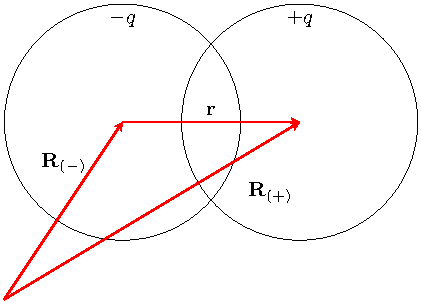
\includegraphics[scale=1.25]{./img/dipole1/dipole1.pdf}
		\caption{Электрический диполь}
	\end{figure}
	Полезная характеристика диполя -- дипольный момент\index{Момент!дипольный}:
	\begin{equation}
		\vec{d}=q\vec{r}.
	\end{equation}
	\begin{equation}
		\vec{d}=q(\vec{R}_{(+)}-\vec{R}_{(-)})=\sum_{(+)} q_i\vec{r}_i + \sum_{(-)} q_k\vec{r}_k=\sum_{\text{по всем}} q_i\vec{r}_i.
	\end{equation}
	Рассмотрим диполь во~внешнем постоянном электрическом поле\index{Поле!постоянное}\index{Поле!электрическое}.
	\begin{figure}[h!]
		\label{fig:dipole2}
		\centering
		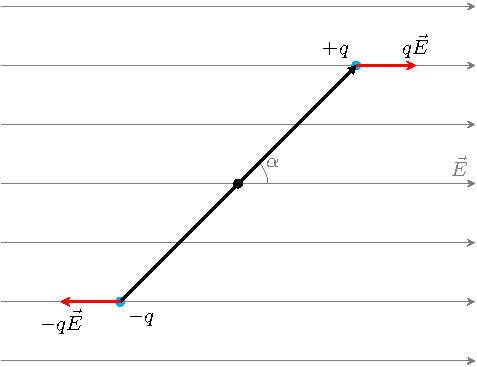
\includegraphics[scale=1.25]{./img/dipole2/dipole2.pdf}
		\caption{Электрический диполь во внешнем постоянном электрическом поле}
	\end{figure}
	Запишем момент сил\index{Момент!сил}, действующий на диполь\index{Диполь!электрический} (рис.~\ref{fig:dipole2}):
		$$M=2F\cdot\frac{l}{2}\sin{\alpha}=Fl\sin{\alpha}=qEl\sin{\alpha}=dE\sin{\alpha},$$
	откуда
	\begin{equation}
		\vec{M}=\vec{d}\times\vec{E}.
	\end{equation}
	На каждый диполь\index{Диполь!электрический} в~электрическом поле\index{Поле!электрическое} действует момент сил\index{Момент!сил}, который ориентирует диполь сонаправленно с~полем.

		\subsection{Энергия диполя во внешнем поле}

		\begin{figure}[h!]
			\label{fig:dipole3}
			\centering
			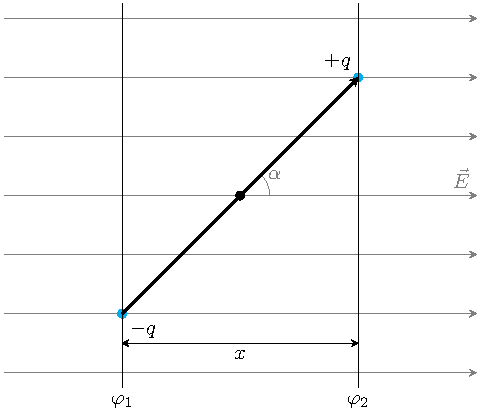
\includegraphics[scale=1.25]{./img/dipole3/dipole3.pdf}
			\caption{Электрический диполь во внешнем постоянном электрическом поле}
		\end{figure}
		Полная потенциальная энергия\index{Энергия!диполя} диполя\index{Диполь!} во внешнем поле (рис.~\ref{fig:dipole3}):
			$$E_{\text{п}}=+q\varphi_2+(-q)\varphi_1=q(\varphi_2-\varphi_1)=-qEx=-qEl\cos{\alpha}=-Ed\cos{\alpha}.$$
		\begin{equation}
			E_{\text{п}}=-\vec{E}\cdot\vec{d}.
		\end{equation}
		Если диполь сонаправлен с~полем, то его энергия наименшая:
			$$\vec{d}\codirect\vec{E}, \quad E_{\text{п}}=-Ed.$$
		Таким образом, сонаправленное положение диполя с внешним полем -- наиболее выгодное.

		\subsection{Электрическое поле диполя}

		\begin{figure}[h!]
			\label{fig:dipole4}
			\centering
			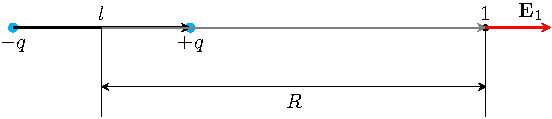
\includegraphics[scale=1.25]{./img/dipole4/dipole4.pdf}
			\caption{Точка 1 на расстоянии $R$ от центра диполя}
		\end{figure}
		Найдем поле, создаваемое диполем в точках 1 и 2 на расстоянии $R$ от центра диполя, если $l\ll R$, где $l$ -- длина диполя (рис.~\ref{fig:dipole4}). Тогда
			$$E_1=k\frac{q}{(R-l/2)^2}-k\frac{q}{(R+l/2)^2}=\frac{kq\left[(R+l/2)^2-(R-l/2)^2\right]}{(R+l/2)^2(R-l/2)^2}=$$
			$$=\frac{2kqRl}{\left(R^2-\left(\cfrac{l}{2}\right)^2\right)^2}.$$
		Пренебрегая длиной диполя по сравнению с $R$, напишем
			$$E_1\simeq\frac{2kqRl}{R^4}=\frac{2kql}{R^3},$$
		\begin{equation}
			E_1\simeq\frac{2kd}{R^3}
		\end{equation}
		Поступим аналогично для точки 2:
		\begin{SCfigure}
			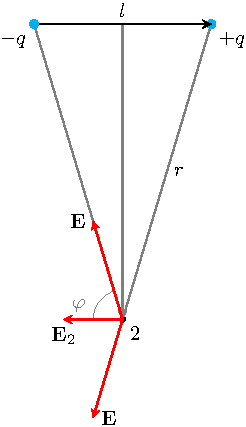
\includegraphics[scale=1.25]{./img/dipole5/dipole5.pdf}
			\caption{Точка 2 на расстоянии $R$ от центра диполя}
		\end{SCfigure}
			$$E_2=2E\cos{\varphi}=-2k\frac{q}{r^2}\cdot\frac{l/2}{r}=-\frac{kd}{r^3}=-\frac{kd}{\left(R^2+\left(\cfrac{l}{2}\right)^2\right)^{3/2}},$$
		\begin{equation}
			E_2\simeq-\frac{kd}{R^3}.
		\end{equation}
		Без доказательства приведем общую формулу:
		\begin{equation}
			\vec{E}=k\frac{3(\vec{d}\cdot\vec{n})\vec{n}-\vec{d}}{R^3} \quad \text{(верно при $l\ll R$)}.
		\end{equation}
		\begin{figure}[h!]
			\label{fig:dipole6}
			\centering
			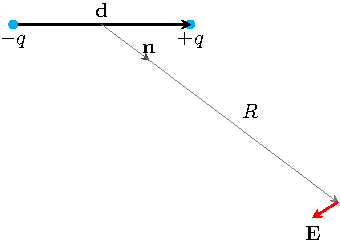
\includegraphics[scale=1.25]{./img/dipole6/dipole6.pdf}
			\caption{Поле диполя в точке на расстоянии $R$}
		\end{figure}
		Этой формулой описывается вся картина поля, создаваемого диполем. Заметим, что оно спадает как $\dfrac{1}{R^3}$.